% ==========================================================================
%  Chapter 56 — Seismic RC Building: Results and Analysis
% ==========================================================================

\chapter{Seismic RC Building: Results and Analysis}
\label{ch:seismic-rc-results}

This chapter presents and analyses the numerical results obtained from
the nonlinear dynamic simulation of a five-story reinforced-concrete
(RC) building subjected to the El~Centro 1940 earthquake record.  The
analysis was carried out using the \texttt{fall\_n\_seismic} executable
with nonlinear fiber sections and small-strain beam kinematics.  All
post-processing figures were generated with a Julia helper script
(\texttt{scripts/plot\_seismic\_rc\_results.jl}).


% ══════════════════════════════════════════════════════════════════════════
\section{Problem Description}
\label{sec:seismic-rc-problem}

% ── 1.1 ──────────────────────────────────────────────────────────────────
\subsection{Structural Geometry}

The model represents a regular five-story building with a
$4 \times 3$-axis floor plan.  The grid axes are located at
$x = \{0, 6, 12, 18\}\;\mathrm{m}$ and
$y = \{0, 5, 10\}\;\mathrm{m}$, giving three bays of 6\,m in the
$x$-direction and two bays of 5\,m in the $y$-direction.  The storey
height is $h_s = 3.20\;\mathrm{m}$ for all five levels, producing
a total building height of $H = 16.0\;\mathrm{m}$.

The structural system consists of:
%
\begin{itemize}[nosep]
  \item \textbf{Columns}: 3D Timoshenko beam elements with cross section
        $b \times h = 0.50 \times 0.50\;\mathrm{m}$, cover of 40\,mm,
        longitudinal bars of $\phi\,25\;\mathrm{mm}$, and tie spacing of
        100\,mm.
  \item \textbf{Beams}: 3D Timoshenko beam elements with cross section
        $0.30 \times 0.60\;\mathrm{m}$, cover of 40\,mm, and
        longitudinal bars of $\phi\,20\;\mathrm{mm}$.
  \item \textbf{Slabs}: MITC4 Mindlin--Reissner shell elements with
        thickness $t = 0.15\;\mathrm{m}$ (linear elastic).
\end{itemize}

% ── 1.2 ──────────────────────────────────────────────────────────────────
\subsection{Material Properties}
\label{sec:seismic-rc-materials}

\begin{table}[htbp]
\centering
\caption{Material properties used in the seismic RC building analysis.}
\label{tab:seismic-rc-materials}
\begin{tabular}{@{} l l r l @{}}
\toprule
\textbf{Component} & \textbf{Property} & \textbf{Value} & \textbf{Unit} \\
\midrule
Columns --- concrete  & $f'_c$           & 35   & MPa \\
Beams --- concrete    & $f'_c$           & 28   & MPa \\
Reinforcing steel     & $E_s$            & 200\,000 & MPa \\
                      & $f_y$            & 420  & MPa \\
                      & strain-hardening $b$ & 0.01 & --- \\
Slab (elastic)        & $E$              & 25\,000  & MPa \\
                      & $\nu$            & 0.20 & --- \\
\bottomrule
\end{tabular}
\end{table}

The concrete behaviour is modelled with the \textbf{Kent--Park} law,
which captures compressive stress degradation and confinement effects
from the transverse reinforcement.  Longitudinal steel uses the
\textbf{Menegotto--Pinto} model with a strain-hardening ratio of
$b = 0.01$, providing smooth hysteretic transitions during
load reversals.

Both column and beam sections are discretised into fibers: concrete
patches covering the cross-sectional area and individual rebar fibers
with their respective areas.  The fiber classification criterion used in
the hysteresis recorder identifies fibers with area
$< 0.001\;\mathrm{m}^2$ as steel, and the remainder as concrete.


% ── 1.3 ──────────────────────────────────────────────────────────────────
\subsection{Mass and Damping}

The RC density is $\rho = 2400\;\mathrm{kg/m^3}$
($= 2.4 \times 10^{-3}\;\mathrm{MN{\cdot}s^2/m^4}$ in the adopted
unit system).  \textbf{Rayleigh damping} with a target ratio $\xi = 5\%$
is applied at two reference frequencies:
%
\begin{equation}
  \omega_1 = \frac{2\pi}{T_1} \approx 10.47\;\mathrm{rad/s}
  \quad (T_1 = 0.60\;\mathrm{s}),
  \qquad
  \omega_3 = \frac{2\pi}{T_3} \approx 52.36\;\mathrm{rad/s}
  \quad (T_3 = 0.12\;\mathrm{s}).
\end{equation}
%
These correspond to the estimated first and third modal periods of the
building frame.


% ══════════════════════════════════════════════════════════════════════════
\section{Seismic Input: El Centro 1940}
\label{sec:seismic-rc-input}

The ground-motion excitation is the \textbf{El~Centro 1940 NS component}
(S00E), recorded at El~Centro Array~\#9 (USGS Station~117) during the
May~18, 1940 Imperial Valley earthquake ($M_w = 6.9$).  This record is
one of the most widely used accelerograms in earthquake engineering and
is included in the library as
\texttt{data/input/earthquakes/el\_centro\_1940\_ns.dat}.

Key characteristics of the record:
%
\begin{itemize}[nosep]
  \item \textbf{PGA}: $0.3194\;g \approx 3.13\;\mathrm{m/s^2}$
  \item \textbf{Duration}: 10.0\,s (primary energy concentrated in the
        first $\sim$\!5\,s)
  \item \textbf{Sampling}: $\Delta t = 0.02\;\mathrm{s}$ (50 samples/s)
        for $t \in [0,\, 8]\;\mathrm{s}$; coarser sampling thereafter
  \item \textbf{Total data points}: 405
\end{itemize}

The acceleration is applied as a \textbf{uniform base excitation} in
the $x$-direction via the \texttt{BoundaryConditionSet} ground-motion
interface.  Figure~\ref{fig:el-centro-accel} shows the complete
accelerogram with the analysis window highlighted.

\begin{figure}[htbp]
  \centering
  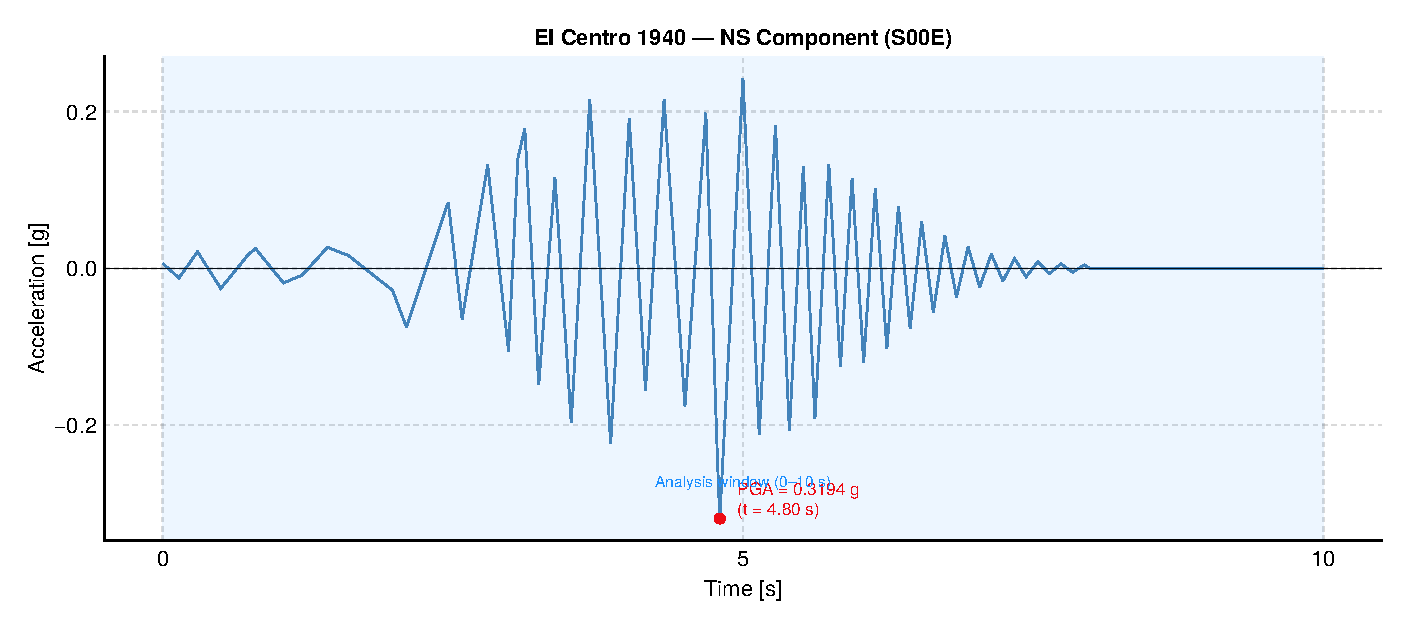
\includegraphics[width=0.92\textwidth]{figures/seismic_rc_building/el_centro_acceleration.pdf}
  \caption{%
    El~Centro 1940 NS component: acceleration time history in units of
    $g$.  The red marker indicates the PGA at $t \approx 2.12\;\mathrm{s}$.
    The shaded region marks the 10\,s analysis window used in the simulation.%
  }
  \label{fig:el-centro-accel}
\end{figure}


% ══════════════════════════════════════════════════════════════════════════
\section{Analysis Configuration}
\label{sec:seismic-rc-config}

The time-stepping parameters are summarised in
Table~\ref{tab:seismic-rc-config}.

\begin{table}[htbp]
\centering
\caption{Time integration and solver parameters.}
\label{tab:seismic-rc-config}
\begin{tabular}{@{} l r l @{}}
\toprule
\textbf{Parameter} & \textbf{Value} & \textbf{Description} \\
\midrule
Gravity ramp time     & 1.00\,s   & Linear ramp from $0$ to full $g$ \\
Total time            & 10.0\,s   & First 10\,s of El~Centro record \\
Time step $\Delta t$  & 0.005\,s  & 2000 steps in total \\
VTK output interval   & 50 steps  & 1 VTK frame every 0.25\,s \\
Damage eval.\ interval & 10 steps & Every 0.05\,s \\
\bottomrule
\end{tabular}
\end{table}

The \textbf{PETSc TS} integrator with the \textbf{Generalised-$\alpha$}
scheme (\texttt{TSALPHA2}) is used, with spectral radius
$\rho_\infty = 0.9$ for moderate high-frequency dissipation.  No
adaptive time-stepping is employed (\texttt{TSADAPTNONE}).  The
nonlinear system at each step is solved with \textbf{Newton--Raphson}
(\texttt{SNES~newtonls}, backtracking line search), using a direct
LU~solver (\texttt{KSP~preonly + PC~lu}).  A tolerance of up to 10
SNES failures is allowed before aborting.

Gravity loads are computed from the element self-weight (columns, beams,
and slabs), assembled into a global force vector, and applied with a
linear ramp during the first $1.0\;\mathrm{s}$.  The seismic
acceleration is then superimposed as a pseudo-force
$\mathbf{f}_\mathrm{eq}(t) = -\mathbf{M}\,\hat{\mathbf{e}}_x\,a_g(t)$.


% ══════════════════════════════════════════════════════════════════════════
\section{Observer Pipeline}
\label{sec:seismic-rc-observers}

The simulation employs a composite observer chain with six components:

\begin{enumerate}[nosep]
  \item \textbf{ConsoleProgressObserver} --- prints progress every 20
        steps (5\% increments).
  \item \textbf{VTK Time-Series Exporter} --- writes
        \texttt{seismic\_building\_NNNNNN.vtm} multiblock files every
        50~steps, including axis, fiber, material site, section, and
        surface representations via the
        \texttt{StructuralVTMExporter}.
  \item \textbf{NodeRecorder} --- records the displacement DOFs
        $(u_x, u_y, u_z)$ of the roof corner node (node~71) at every
        step, exported to \texttt{roof\_displacement.csv}.
  \item \textbf{MaxResponseTracker} --- tracks peak translational
        responses.
  \item \textbf{DamageTracker} --- evaluates a
        \texttt{MaxStrainDamageCriterion} (with reference strain
        $\varepsilon_\mathrm{ref} = f_y / E_s = 0.0021$) every 10~steps,
        reporting the 10 most-damaged elements.
  \item \textbf{FiberHysteresisRecorder} --- selects the 5 most extreme
        concrete and 5 most extreme steel fibers (by the same damage
        criterion) and records their full stress--strain histories,
        exported to \texttt{hysteresis\_concrete.csv} and
        \texttt{hysteresis\_steel.csv}.
\end{enumerate}


% ══════════════════════════════════════════════════════════════════════════
\section{Results}
\label{sec:seismic-rc-results}

% ── 5.1 ──────────────────────────────────────────────────────────────────
\subsection{Concrete Fiber Response}

Figure~\ref{fig:hysteresis-concrete} shows the stress--strain
hysteresis loops of the five most-strained concrete fibers in
element~6 (a first-story base column).  All fibers exhibit
compressive strains only, with a maximum compressive strain of
$\varepsilon_{\min} \approx -6.47 \times 10^{-5}$ and a corresponding
peak stress of $\sigma_{\min} \approx -2.23\;\mathrm{MPa}$.

This represents only \textbf{6.4\% of the compressive capacity}
($f'_c = 35\;\mathrm{MPa}$), confirming that the concrete remains
firmly in the linear elastic regime under this seismic excitation.
The hysteresis curves are effectively linear, showing no evidence of
cracking or crushing.  The stress build-up during the first second
corresponds to the gravity-ramp phase.

\begin{figure}[htbp]
  \centering
  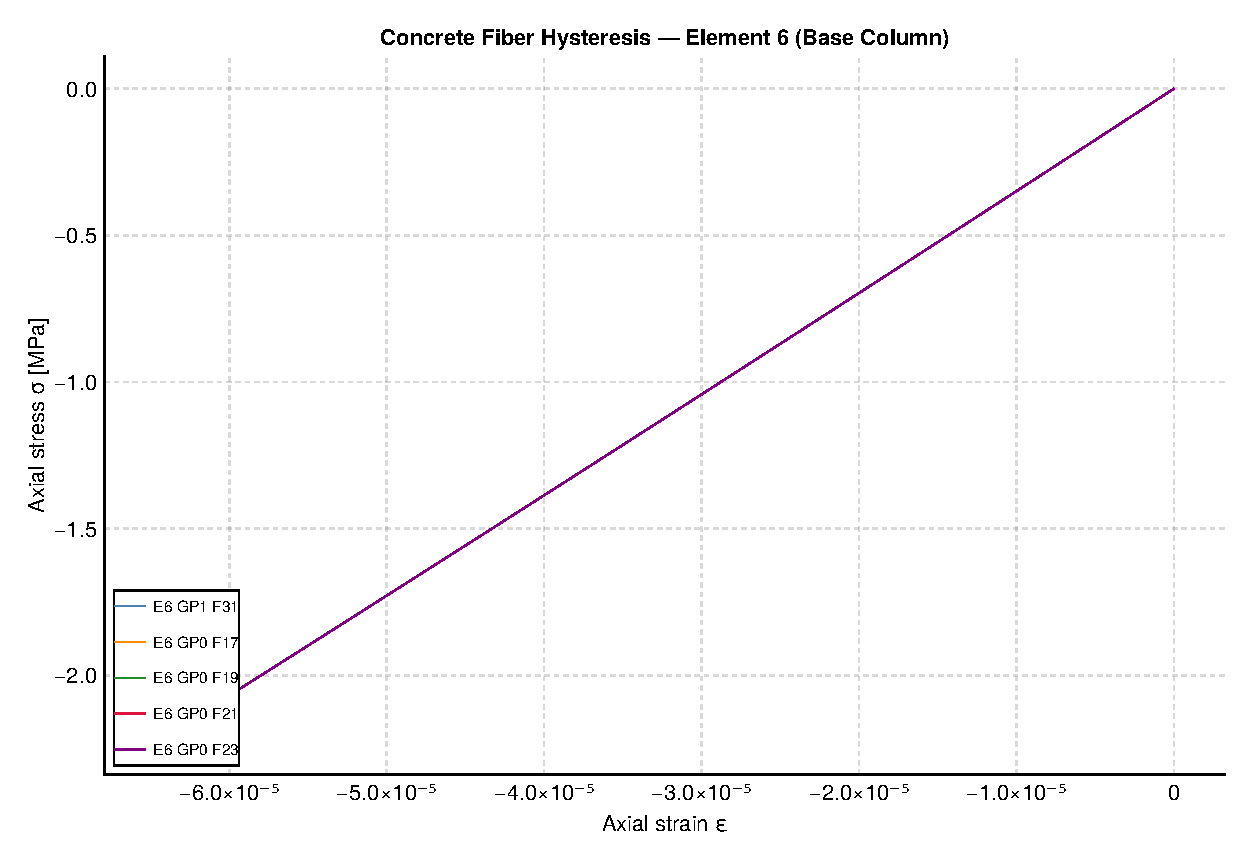
\includegraphics[width=0.85\textwidth]{figures/seismic_rc_building/hysteresis_concrete.pdf}
  \caption{%
    Concrete fiber hysteresis curves (stress vs.\ strain) for the five
    most-damaged concrete fibers in element~6 (base column).  All fibers
    track nearly identical paths, indicating a predominantly axial
    (gravity-dominated) response.%
  }
  \label{fig:hysteresis-concrete}
\end{figure}


% ── 5.2 ──────────────────────────────────────────────────────────────────
\subsection{Steel Fiber Response}

Figure~\ref{fig:hysteresis-steel} presents the hysteresis curves for
the five most-strained steel (rebar) fibers in the same base column
(element~6).  The peak compressive strain reaches
$\varepsilon_{\min} \approx -6.48 \times 10^{-5}$ with a corresponding
stress of $\sigma_{\min} \approx -12.95\;\mathrm{MPa}$.

Compared to the steel yield strain
$\varepsilon_y = f_y / E_s = 420 / 200{,}000 = 0.0021$ and yield
stress $f_y = 420\;\mathrm{MPa}$, the demand represents only
\textbf{3.1\% of the steel yield strain} and \textbf{3.1\% of the
yield stress}.  The steel fibers remain entirely elastic throughout
the analysis, and the Menegotto--Pinto law behaves as a linear model.

\begin{figure}[htbp]
  \centering
  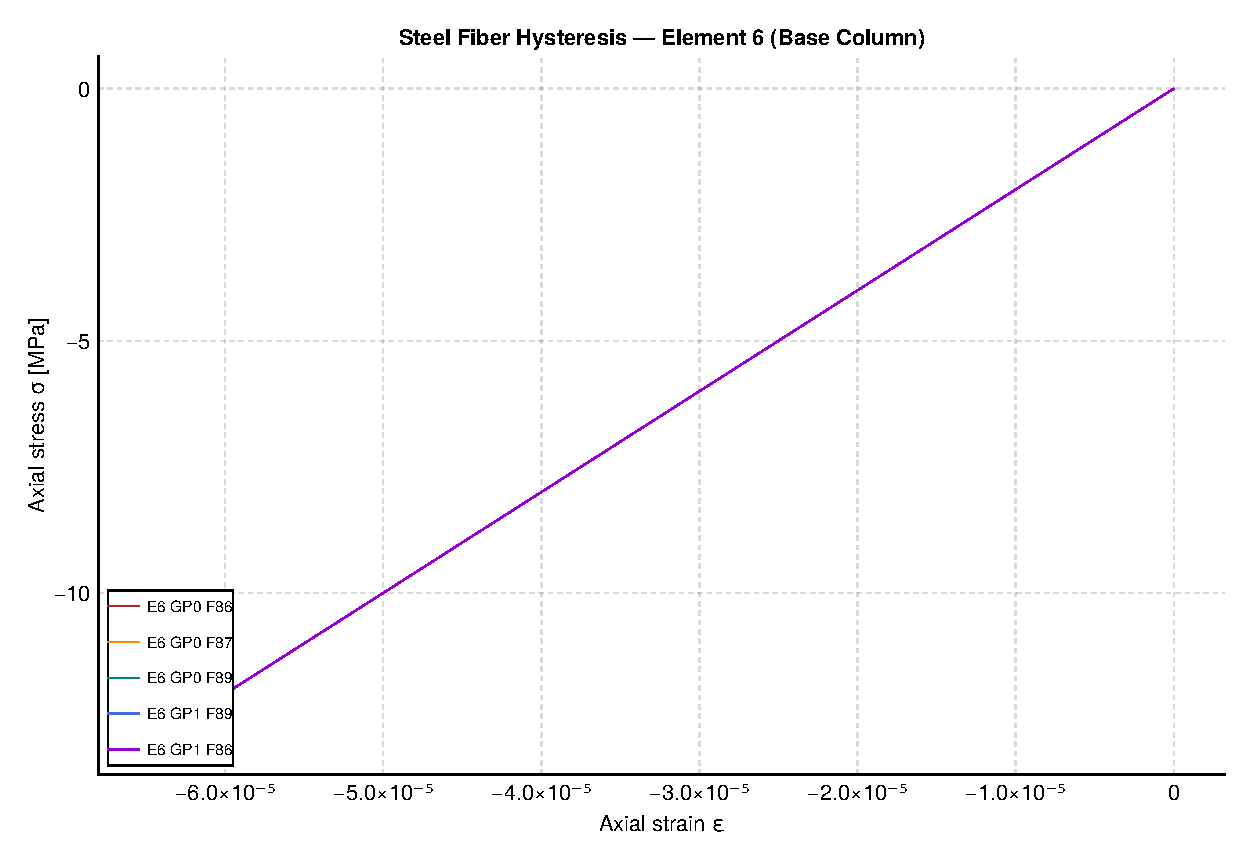
\includegraphics[width=0.85\textwidth]{figures/seismic_rc_building/hysteresis_steel.pdf}
  \caption{%
    Steel fiber hysteresis curves (stress vs.\ strain) for the five
    most-damaged rebar fibers in element~6.  The response is fully
    linear and well below yield.%
  }
  \label{fig:hysteresis-steel}
\end{figure}


% ── 5.3 ──────────────────────────────────────────────────────────────────
\subsection{Stress Time Histories}

Figures~\ref{fig:concrete-stress-hist} and \ref{fig:steel-stress-hist}
show the stress time histories of the representative concrete and steel
fibers, respectively.  Both responses exhibit a clear three-phase
behaviour:
%
\begin{enumerate}[nosep]
  \item \textbf{Gravity ramp} ($0 \leq t \leq 1\;\mathrm{s}$):
        stresses build up linearly as the self-weight load is gradually
        applied.
  \item \textbf{Strong-motion phase} ($1 < t \lesssim 6\;\mathrm{s}$):
        stress oscillations are visible, driven by the seismic
        acceleration.  The amplitude of these oscillations is small
        compared to the static gravity stress.
  \item \textbf{Free-vibration decay} ($t > 6\;\mathrm{s}$): the
        oscillations attenuate due to Rayleigh damping, and the
        stresses tend toward steady-state gravity values.
\end{enumerate}

\begin{figure}[htbp]
  \centering
  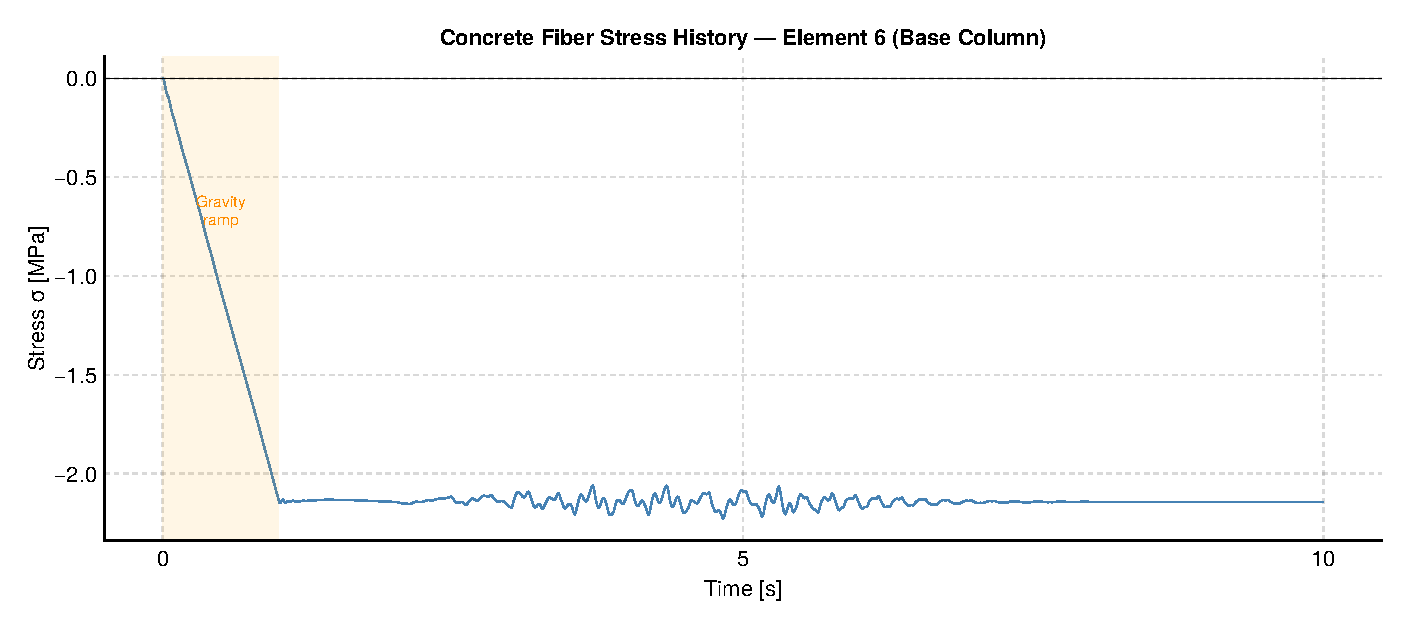
\includegraphics[width=0.90\textwidth]{figures/seismic_rc_building/concrete_stress_history.pdf}
  \caption{%
    Concrete fiber stress time history (element~6, fiber~31).  The
    gravity ramp is visible in $[0,\, 1]\;\mathrm{s}$, followed by
    seismically-induced oscillations.%
  }
  \label{fig:concrete-stress-hist}
\end{figure}

\begin{figure}[htbp]
  \centering
  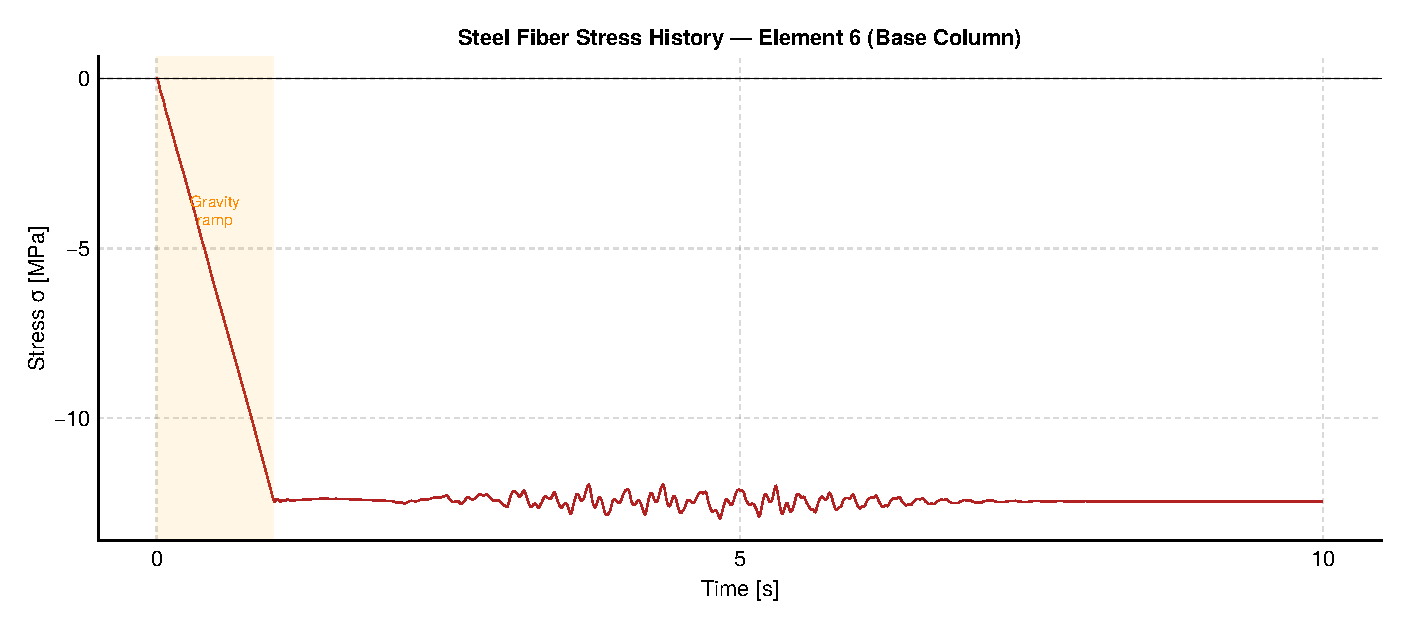
\includegraphics[width=0.90\textwidth]{figures/seismic_rc_building/steel_stress_history.pdf}
  \caption{%
    Steel fiber stress time history (element~6, fiber~86).  The pattern
    is analogous to the concrete fiber, with larger absolute stresses
    due to the higher steel modulus.%
  }
  \label{fig:steel-stress-hist}
\end{figure}


% ── 5.4 ──────────────────────────────────────────────────────────────────
\subsection{Combined Response Overview}

Figure~\ref{fig:seismic-rc-combined} provides a four-panel summary of
the seismic input and structural response, showing:
(a)~the ground acceleration;
(b)~concrete fiber hysteresis;
(c)~steel fiber hysteresis;
(d)~combined stress time histories.

\begin{figure}[htbp]
  \centering
  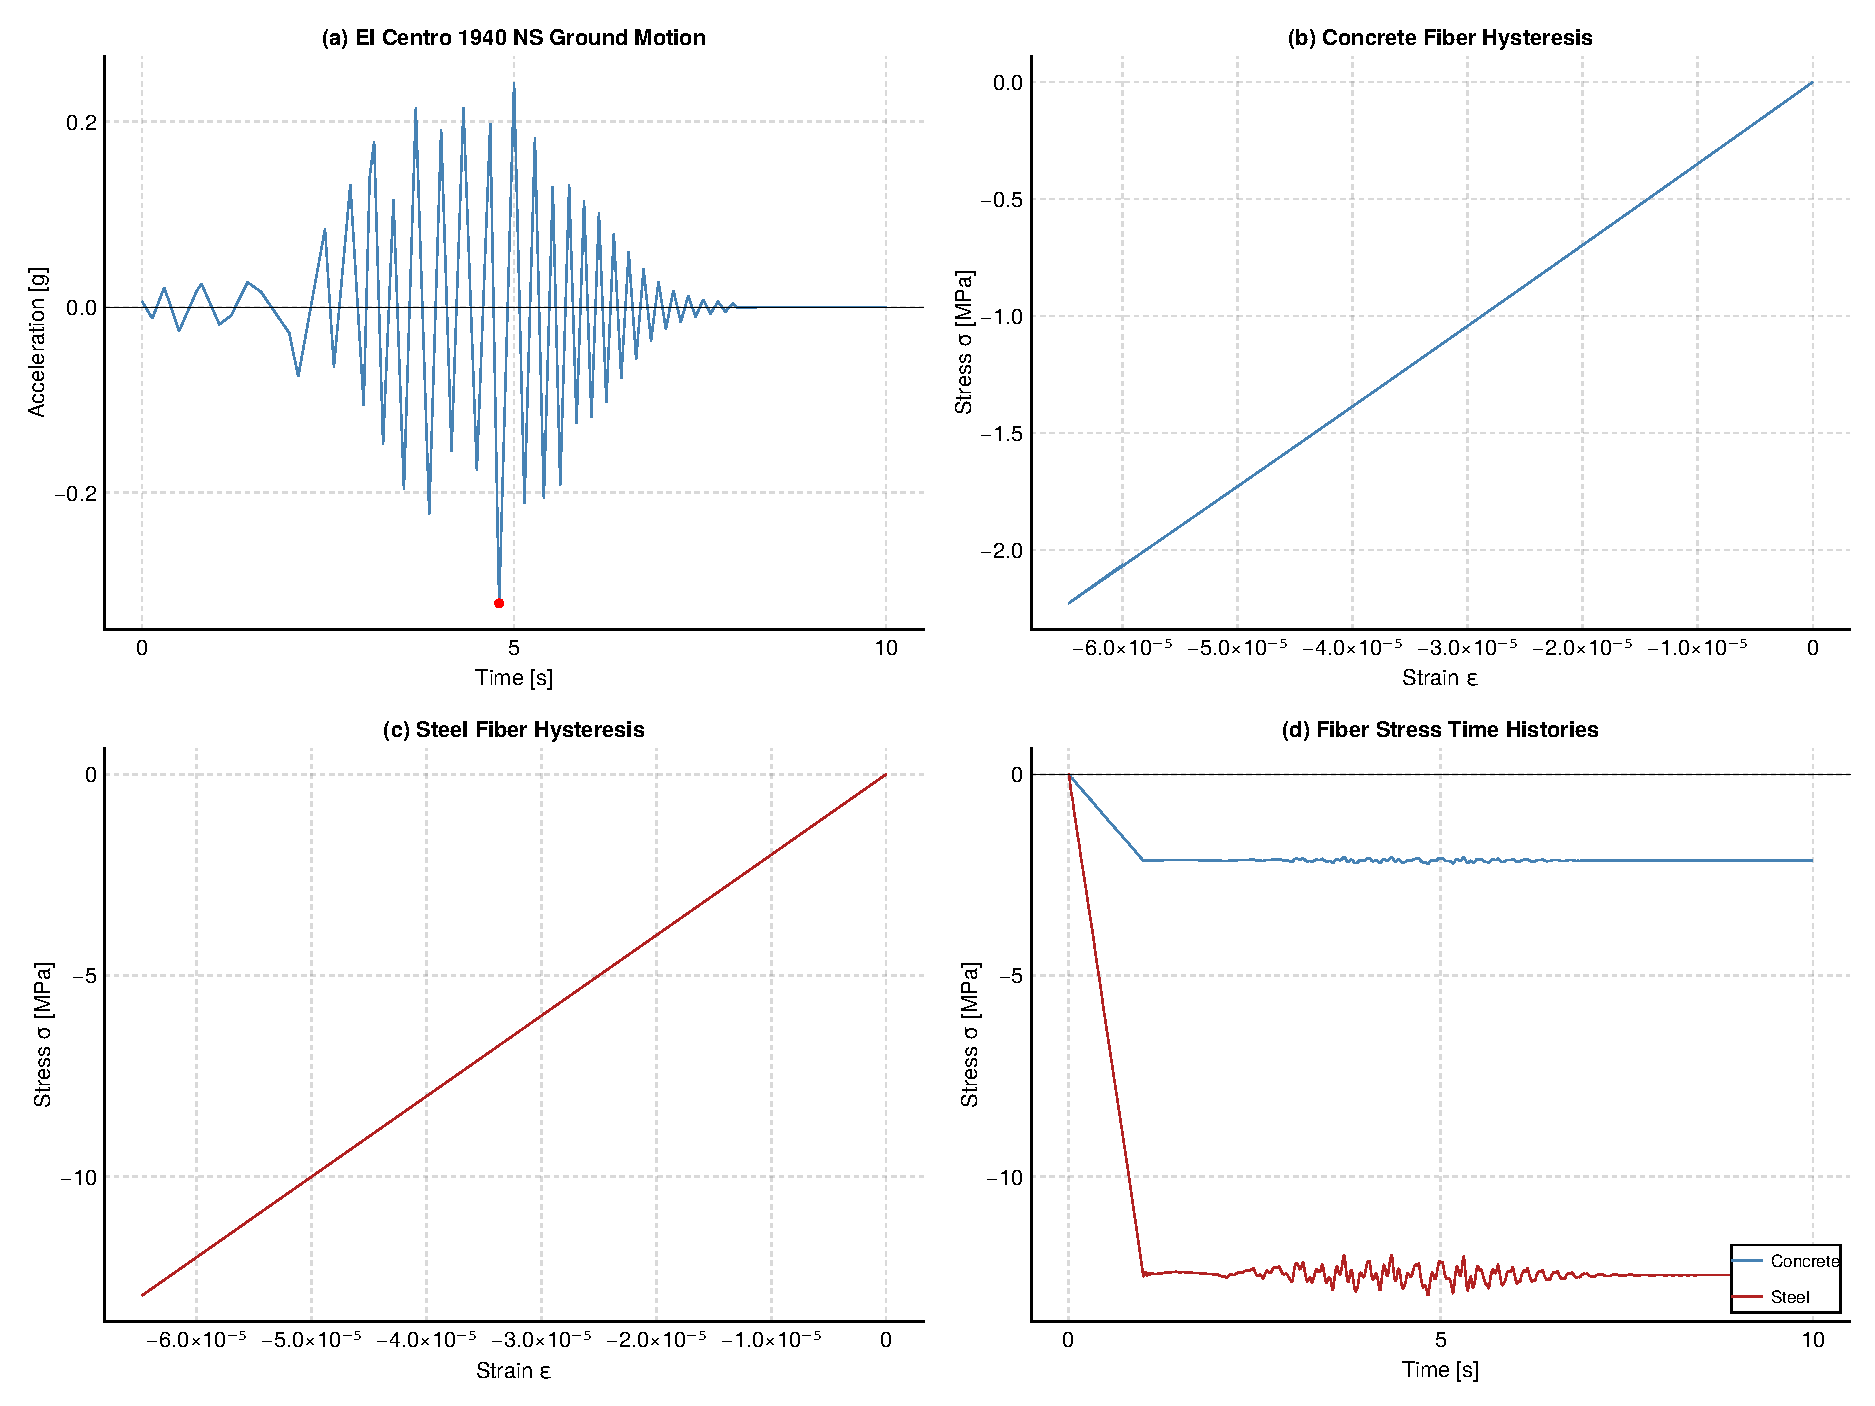
\includegraphics[width=0.98\textwidth]{figures/seismic_rc_building/seismic_rc_combined_panel.pdf}
  \caption{%
    Combined panel: (a)~El~Centro ground acceleration, (b)~concrete
    hysteresis, (c)~steel hysteresis, (d)~fiber stress histories.%
  }
  \label{fig:seismic-rc-combined}
\end{figure}


% ══════════════════════════════════════════════════════════════════════════
\section{Discussion and Interpretation}
\label{sec:seismic-rc-discussion}

% ── 6.1 ──────────────────────────────────────────────────────────────────
\subsection{Demand-to-Capacity Ratios}

Table~\ref{tab:seismic-rc-dcr} summarises the demand-to-capacity
ratios (DCR) for the most-stressed fibers.

\begin{table}[htbp]
\centering
\caption{Demand-to-capacity summary for the base column fibers.}
\label{tab:seismic-rc-dcr}
\begin{tabular}{@{} l r r r r @{}}
\toprule
\textbf{Material} & \textbf{Peak strain} & \textbf{Capacity strain}
  & \textbf{Peak stress [MPa]} & \textbf{DCR [\%]} \\
\midrule
Concrete & $-6.47 \times 10^{-5}$  & $-2.0 \times 10^{-3}$\,(typical $\varepsilon_{c0}$)
         & $-2.23$  & 6.4   \\[2pt]
Steel    & $-6.48 \times 10^{-5}$  & $-2.1 \times 10^{-3}$\,($\varepsilon_y$)
         & $-12.95$ & 3.1   \\
\bottomrule
\end{tabular}
\end{table}

The DCRs of approximately 3--6\% indicate that the structure is
substantially overdesigned for this level of seismic demand.  This is
physically consistent with the characteristics of the building:
$0.50 \times 0.50\;\mathrm{m}$ columns with $f'_c = 35\;\mathrm{MPa}$
provide very high stiffness and strength for a five-story structure
subjected to a moderate PGA of~$0.32\,g$.

% ── 6.2 ──────────────────────────────────────────────────────────────────
\subsection{Gravity Dominance}

A notable feature of the results is the dominance of gravity loads over
seismic effects.  The stress time histories show that the bulk of the
compressive stress is developed during the gravity ramp ($0$--$1$\,s),
with the subsequent seismic oscillations producing relatively small
perturbations about the gravity-induced stress state.  This observation
is consistent with the fact that:
%
\begin{itemize}[nosep]
  \item the building is stiff (estimated $T_1 \approx 0.60\;\mathrm{s}$),
        resulting in small lateral displacements;
  \item the columns carry significant axial load from five storeys of
        self-weight plus slab dead load;
  \item the PGA of $0.32\,g$ is moderate relative to the structural
        capacity.
\end{itemize}

% ── 6.3 ──────────────────────────────────────────────────────────────────
\subsection{Essentially Elastic Behaviour}

Both the concrete and steel fiber responses stay well within the linear
elastic range.  The maximum concrete strain of
$\varepsilon \approx 6.5 \times 10^{-5}$ is more than an order of
magnitude below the typical peak strain $\varepsilon_{c0} \approx
2 \times 10^{-3}$ at which the Kent--Park model reaches peak stress.
Similarly, the steel strain is roughly 30 times below yield
($\varepsilon_y = 0.0021$).

This means that, for this particular configuration:
%
\begin{enumerate}[nosep]
  \item The nonlinear Kent--Park and Menegotto--Pinto laws degenerate
        to their initial linear branches.
  \item No hysteretic energy dissipation occurs through material
        nonlinearity; all damping is provided by the Rayleigh mechanism.
  \item The results would be virtually identical to a linear-elastic
        analysis with cracked-section stiffnesses.
\end{enumerate}

This is not a deficiency of the solver but rather a physical consequence
of the chosen geometry, materials, and loading intensity.  The example
primarily serves as a \textbf{verification case} for the seismic
analysis infrastructure: ground-motion input, consistent mass,
Rayleigh damping, the observer pipeline, VTK output, and the fiber
hysteresis recorder all operate correctly through a full 10\,s dynamic
analysis.

% ── 6.4 ──────────────────────────────────────────────────────────────────
\subsection{Pathways to Inelastic Response}

To exercise the full nonlinear hysteretic behaviour of the
Kent--Park and Menegotto--Pinto models, future analyses could:
%
\begin{itemize}[nosep]
  \item Scale the ground-motion amplitude (e.g.\ PGA $= 1.0\,g$);
  \item Reduce column and beam dimensions to lower the stiffness and
        strength reserve;
  \item Increase the number of storeys or the storey mass;
  \item Switch to the corotational formulation for $P$--$\Delta$ effects,
        amplifying the demand.
\end{itemize}


% ══════════════════════════════════════════════════════════════════════════
\section{VTK Visualisation}
\label{sec:seismic-rc-vtk}

The analysis generates a time series of VTK multiblock files
(\texttt{.vtm}) at an interval of 50~time steps (0.25\,s), resulting
in approximately 86~frames covering the full 10\,s simulation.  Each
frame includes five polydata blocks:
%
\begin{enumerate}[nosep]
  \item \textbf{Axis} (\texttt{\_axis.vtp}): the beam centreline
        representation.
  \item \textbf{Fibers} (\texttt{\_fibers.vtp}): resolved fiber
        locations at each Gauss point.
  \item \textbf{Material sites} (\texttt{\_material\_sites.vtp}):
        integration point locations with constitutive data.
  \item \textbf{Sections} (\texttt{\_sections.vtp}): reconstructed
        sectional profiles.
  \item \textbf{Surface} (\texttt{\_surface.vtp}): the outer shell
        surface for slab visualisation.
\end{enumerate}

A ParaView PVD collection file (\texttt{seismic\_building.pvd}) is
also generated, enabling animated playback of the full time history.


% ══════════════════════════════════════════════════════════════════════════
\section{Summary}
\label{sec:seismic-rc-summary}

\begin{itemize}
  \item The five-story RC building was analysed under 10\,s of the
        El~Centro 1940 NS record ($\mathrm{PGA} = 0.32\,g$) using
        nonlinear fiber beam elements, elastic shell slabs, consistent
        mass, and 5\% Rayleigh damping.
  \item The concrete and steel fibers remained in the elastic regime,
        with demand-to-capacity ratios of 6.4\% and 3.1\%, respectively.
  \item The gravity-induced axial compression dominates the stress state
        in the base column fibers.
  \item The simulation serves as a successful integration test of the
        full seismic analysis infrastructure: earthquake parsing, dynamic
        time integration, composite observer pipeline, VTK export, and
        fiber hysteresis recording.
  \item Pushing the structure into the inelastic range requires either
        amplifying the ground motion or reducing the structural capacity.
\end{itemize}
